\chapter{Interface K8s Cluster and GitLab-OST}

\section{Overview}
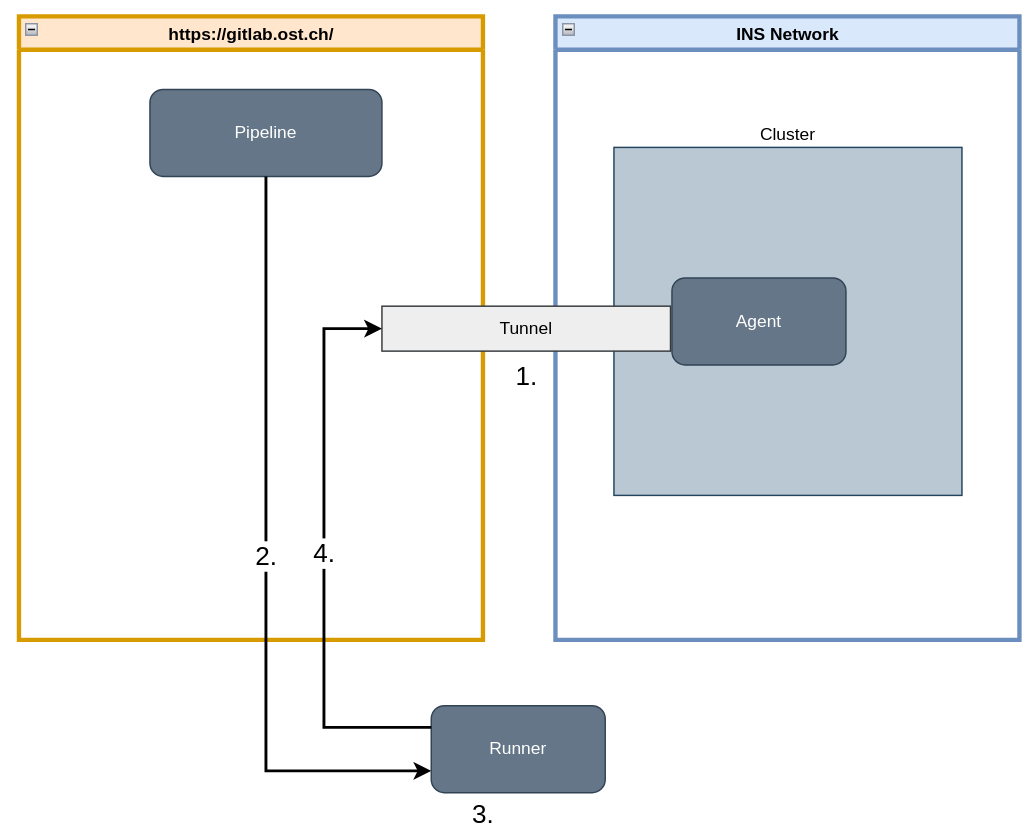
\includegraphics[height=12cm]{resources/k8s_including_in_gitlab-ost.png}
\begin{enumerate}
    \item The \textit{Agent} creates a \textit{Tunnel} from the INS network to the gitlab.ost.ch network.
    \item The \textit{Pipeline} triggers the \textit{Runner} to run the cluster commands.
    \item The \textit{Runner} starts the docker.
    \item The \textit{Runner} gets access to the \textit{tunnel endpoint} via the gitlab.ost.ch network and runs the cluster commands now at the cluster.
\end{enumerate}

\noindent The figure above shows how the Kubernetes cluster and GitLab are combined. GitLab and the cluster are in two different networks,  GitLab is placed in the OST network and the Kubernetes cluster is deployed in the INS network.

Only the \textit{Agent} inside the INS network can create the \textit{Tunnel} to the gitlab.ost.ch network. Nobody from the gitlab.ost.ch network can deploy the \textit{Tunnel} by themself.

The \textit{Runner} is independent of the location, so it does not depend on the network where you place the \textit{Runner}.

\section{Installation Agent in GitLab}
\begin{enumerate}
    \item Add the Kubernetes cluster in the GitLab project, it's important to add this configuration file at the correct path: `.gitlab/agents/ins-cluster-agent/ins-epj.yaml`
    \item Got to the \textbf{Infrastructure -> Kubernetes cluster} tab and install there a new agent (choose the ins-cluster-agent in the drop down menu)
    \item Safe the token! (Our Token: r8J8f3ve-DsU-v8cmrRSZx\_-atYyJqVCyePyk7zVCvSADy5-qg)
    \item Run the docker installation command from the popup window in you CLI (you need first to install docker locally) \newline
    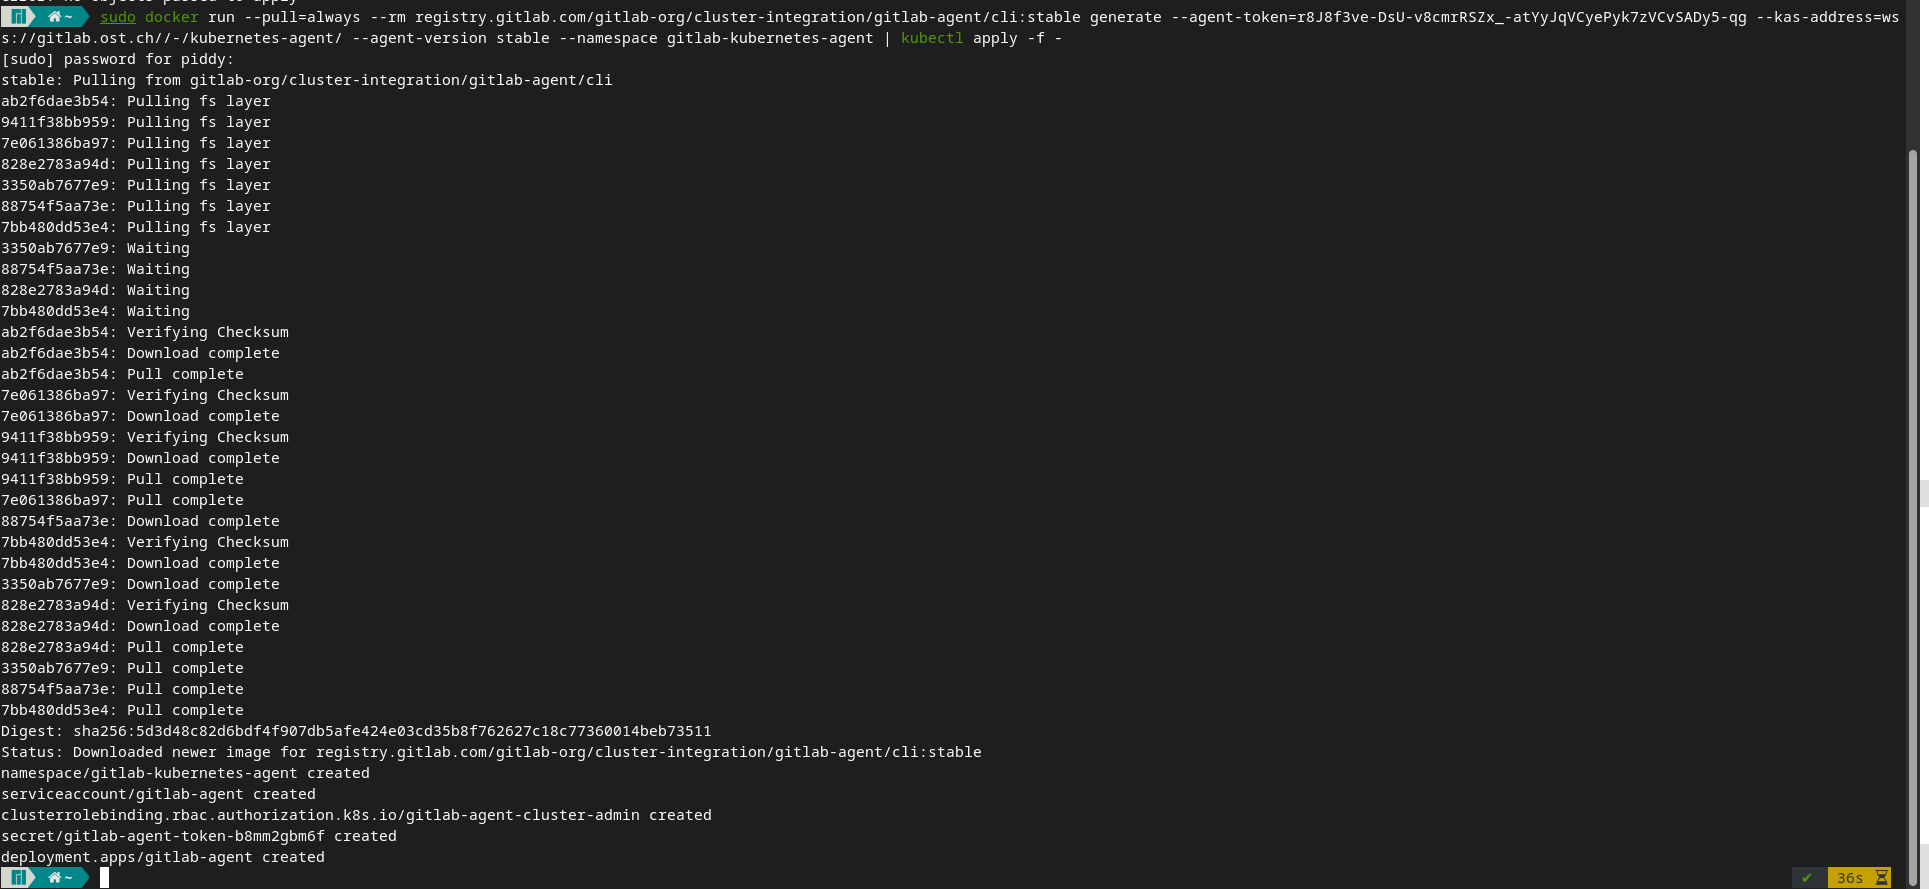
\includegraphics[height=5cm]{resources/agent-installation.png}
    \item Check if the connection in the GitLab is working \newline
    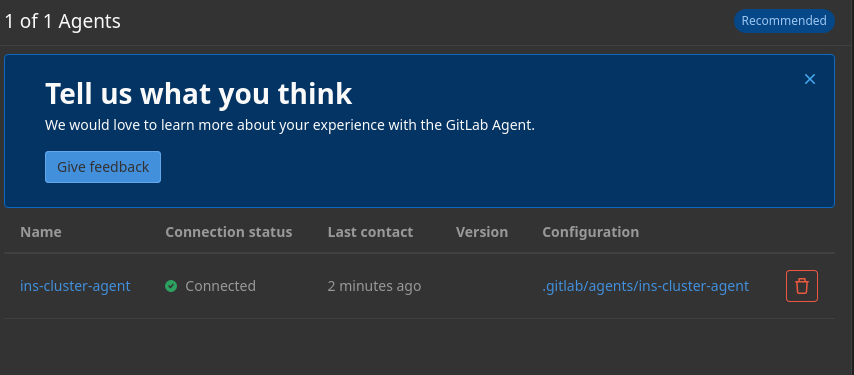
\includegraphics[height=5cm]{resources/ins-cluster-agent-connection.png}
    \item Check if the Cluster is running with the command kubectl config view (the output should be your agent configuration file) \newline
    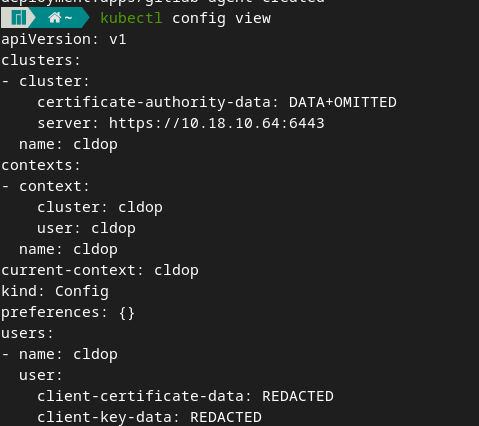
\includegraphics[height=5cm]{resources/ins-cluster-agent-accessing-cluster-test.png}
    \item update you .gitlab-ci.yml file to run kubectl commands
    \item update the agent configuration file for authorize the agent to access the project
\end{enumerate}